\section{Quark/Antiquark gluon emission kernel}


\begin{figure}[ht!]
\centering
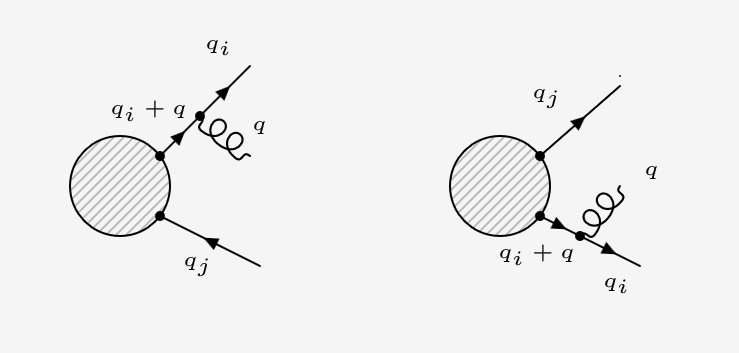
\includegraphics[width=0.85\textwidth]{images/qqg-diagrams.png}
\end{figure}

\subsection{qg-$\bar{q}$}

\begin{figure}[h!]
\centering
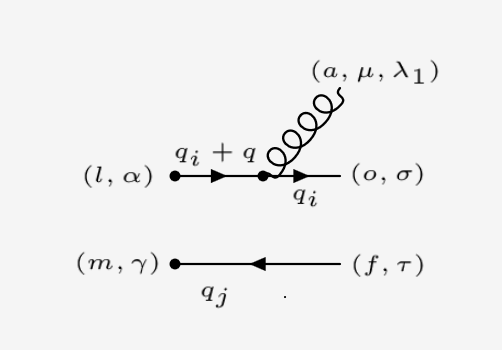
\includegraphics[width=0.85\textwidth]{images/qgqbarM.png}
\end{figure}

\begin{equation}
M_1 = [{\bar{u}}_{\sigma}(q_i) (-ig_s \gamma^{\mu}\times {[T^a]_o}^l)  \frac{i(\not{q_i} + q)}{(q_i + q)^2} {\varepsilon^{\lambda_1}}_{\mu} (q)]\: [{v}_{\tau}(q_j)]
\end{equation}

\begin{figure}[h!]
\centering
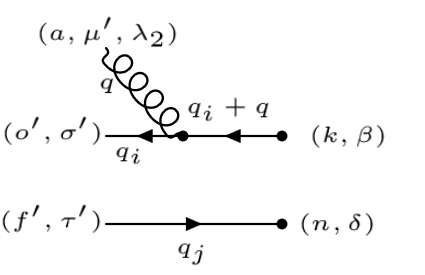
\includegraphics[width=0.85\textwidth]{images/qgqbarMDega.png}
\end{figure}

\begin{equation}
{M_1}^{\dagger} = [\frac{-i(\not{q_i} + \not{q})}{(q_i + q)^2} \:  (ig_s \gamma^{{\mu}^{\prime}}\times {[T^b]_{o\:^{\prime}}}^k) \: u_{{\sigma}^{\prime}}(q_i) \: {\varepsilon^{\lambda_2}}_{{\mu}^{\prime}} (q)][{\bar{v}}_{{\tau}^{\prime}}(q_j)]
\end{equation}

\begin{figure}[h!]
\centering
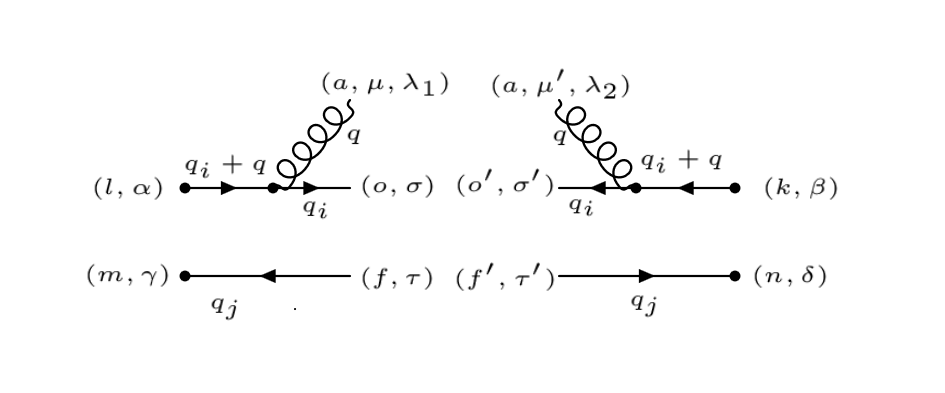
\includegraphics[width=0.85\textwidth]{images/qgqbarMSquer.png}
\end{figure}

\begin{equation}
\begin{split}
|M_1|^2=M_1\:{\color[RGB]{255,0,0} {M_1}^{\dagger}} = [{\bar{u}}_{\sigma}(q_i)\: (-ig_s \gamma^{\mu}\times {[T^a]_o}^l) \: \frac{i(\not{q_i} + q)}{(q_i + q)^2}\:\: {\varepsilon^{\lambda_1}}_{\mu} (q)] [{v}_{\tau}(q_j)]\: \\
\quad\quad\quad\quad\quad\quad\quad\quad\:\:{\color[RGB]{255,0,0}[\frac{-i(\not{q_i} + \not{q})}{(q_i + q)^2} \:  (ig_s \gamma^{{\mu}^{\prime}}\times {[T^b]_{o\:^{\prime}}}^k) \: u_{{\sigma}^{\prime}}(q_i) \: {{\varepsilon^{\lambda_2}}_{{\mu}^{\prime}}}^* (q)][{\bar{v}}_{{\tau}^{\prime}}(q_j)]}
\end{split}
\end{equation}


\begin{equation}
\begin{split}
|M_1|^2=[\frac{-i(\not{q_i} + \not{q})}{(q_i + q)^2} \:
 \:  (ig_s \gamma^{{\mu}^{\prime}}\times {[T^b]_{o\:^{\prime}}}^k) \: {\bar{u}}_{\sigma}(q_i)\:u_{{\sigma}^{\prime}}(q_i) \: {{\varepsilon^{\lambda_2}}_{{\mu}^{\prime}}^* (q) {\varepsilon^{\lambda_1}}_{\mu} (q)} \\
\times (-ig_s \gamma^{\mu}\times {[T^a]_o}^l) \: \frac{i(\not{q_i} + q)}{(q_i + q)^2} ]
[{\bar{v}}_{{\tau}^{\prime}}(q_j) {v}_{\tau}(q_j)]
\end{split}
\end{equation}

and after sum over the lorenz index $({\sigma},{\sigma}^{\prime})$ and $({\tau},{\tau}^{\prime})$ and unsing the spin addition relation:
 
\begin{equation}
\begin{split}
\displaystyle\sum\limits_{{\sigma},{\sigma}^{\prime}} {\bar{u}}_{\sigma}(q_i)\:u_{{\sigma}^{\prime}}(q_i) = \not{q_i},\\
\displaystyle\sum\limits_{{\tau},{\tau}^{\prime}} {\bar{v}}_{\tau}(q_j)\:v_{{\tau}^{\prime}}(q_j) = \not{q_j}
\end{split}
\end{equation}
and sum over polarization index $({\lambda_{1}},{\lambda}_{2})$ :
\begin{equation}
\begin{split}
 \displaystyle\sum\limits_{{\mu},{\mu}^{\prime}} {{\varepsilon^{\lambda_2}}_{{\mu}^{\prime}}^* (q) {\varepsilon^{\lambda_1}}_{\mu} (q)} = -g_{{\mu}{\mu}^{\prime}}
\end{split}
\end{equation}

\begin{equation}
\begin{split}
|M_1|^2=\frac{-g_s^2  {[T^b]_{o\:^{\prime}}}^k \: {[T^a]_o}^l }{(q_i + q)^2 (q_i + q)^2}
[(\not{q_i} + \not{q}) \:
 \:  \gamma^{{\mu}^{\prime}} \: \not{q_i} \: g_{{{\mu}^{\prime}}{\mu}} 
\gamma^{\mu} \: (\not{q_i} + q)]
[\not{q_j}]
\end{split}
\end{equation}

from here and after contraction between all indices we can actually make statements about the last result.
\begin{equation}
\begin{split}
|M_1|^2=\frac{-g_s^2  {[T^b]_{o\:^{\prime}}}^k \: {[T^a]_o}^l }{(q_i + q)^2 (q_i + q)^2}
[(\not{q_i} + \not{q}) \:
 \:  \gamma^{{\mu}^{\prime}} \: \not{q_i} \: 
\gamma_{{\mu}^{\prime}} \: (\not{q_i} + q)]
[\not{q_j}]
\end{split}
\end{equation}

In other words we expect the tree level diagram from LO and a number:
\begin{figure}[h!]
\centering
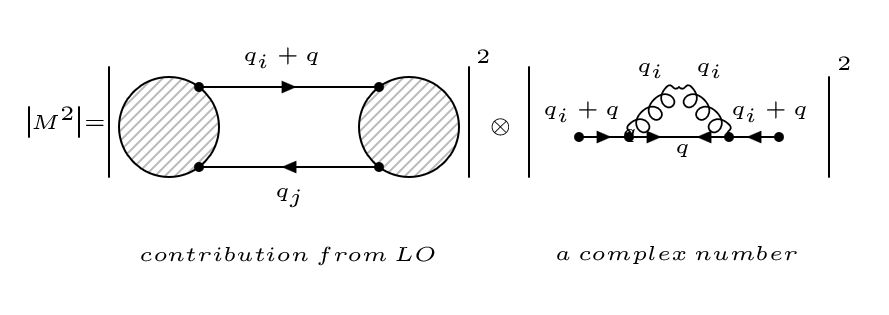
\includegraphics[width=0.85\textwidth]{images/expectationqg-qbar.png}
\end{figure}
Which means:\\
\begin{equation}
\begin{split}
|M_1|^2=\frac{-g_s^2  {[T^b]_{o\:^{\prime}}}^k \: {[T^a]_o}^l }{(q_i + q)^2 (q_i + q)^2}
[\not{P_i}]
[\not{P_j}]\:\otimes \: {\color[RGB]{255,0,0} (a\: complex\: number)}
\end{split}
\end{equation}  
Let's calculate the contribution and compare the final result with this expectation:
\begin{equation}
\begin{split}
N=: \gamma^{{\mu}^{\prime}} \not{q_i} \: \gamma_{{\mu}^{\prime}} = {q_{i\sigma}} \: \gamma^{{\mu}^{\prime}} \gamma^{\sigma} \:\: \gamma_{{\mu}^{\prime}}\\
={q_{i\sigma}} \: (\lbrace{\gamma^{{\mu}^{\prime}}}, {\gamma^{\sigma}}\rbrace \: - {\gamma^{\sigma}}{\gamma^{{\mu}^{\prime}}})\gamma_{{\mu}^{\prime}}\\
={q_{i\sigma}} \: 2g^{{{\mu}^{\prime}}{\sigma}} \: \gamma_{{\mu}^{\prime}} \: - \:d\:{\gamma^{\sigma}}\\
=(2-d) \not{q_i}
\end{split}
\end{equation}

\begin{equation}
\begin{split}
|M_1|^2=-(2-d)\:\frac{g_s^2  {[T^b]_{o\:^{\prime}}}^k \: {[T^a]_o}^l }{(q_i + q)^2 (q_i + q)^2}
[(\not{q_i} + \not{q}) \:
 \:\not{q_i} \: 
 \: (\not{q_i} + q)]
[\not{q_j}]
\end{split}
\end{equation}

\begin{equation}
\begin{split}
|M_1|^2=-(2-d)\:\frac{g_s^2  {[T^b]_{o\:^{\prime}}}^k \: {[T^a]_o}^l }{(q_i + q)^2 (q_i + q)^2}
[\not{q_i} \not{q_i} \not{q_i} \: + \: \not{q_i} \not{q_i} \not{q} \: + \: \not{q} \not{q_i} \not{q_i} \:+\: \not{q} \not{q_i} \not{q}]
[\not{q_j}]
\end{split}
\end{equation}

For the momenta are on-shell which means:
\begin{equation}
\begin{split}
\not{q_i}\not{q_i} = {q_i}= m^2\\
\not{q}\not{q} = {q}= m^2\\
\not{q_j}\not{q_j} = {q_j}= m^2
\end{split}
\end{equation}

we can first neglect the mass of patrons and ignore each term with $ \not{q_i}\not{q_i} $ and  $ \not{q}\not{q} $ as well.

\begin{equation}
\begin{split}
|M_1|^2=-(2-d)\:\frac{g_s^2  {[T^b]_{o\:^{\prime}}}^k \: {[T^a]_o}^l }{(2q_i q)(2q_i q)}
[\not{q} \not{q_i} \not{q}]
[\not{q_j}]
\end{split}
\end{equation}

\begin{equation}
\begin{split}
L=\not{q} \not{q_i} \not{q} =\not{q}[{q_{i\sigma}} q_{\mu} \: (\lbrace{\gamma^{\mu}}, {\gamma^{\sigma}}\rbrace - {\gamma^{\sigma}}{\gamma^{\mu}})]\\ 
\not{q}[2{q_{i}}^{\mu} q_{\mu} - {q_{i\sigma}}q_{\mu}{\gamma^{\mu}}{\gamma^{\sigma}}\\
=\not{q} (2q_i q)-q_{\mu}{q_{i\sigma}}q_{\mu}[{\gamma^{\mu}}{\gamma^{\mu}}{\gamma^{\sigma}}]\\
=\not{q} (2q_i q)-q_{\mu}{q_{i\sigma}}q_{\mu}[\frac{{\gamma^{\mu}}{\gamma^{\mu}}}{2} +\frac{{\gamma^{\mu}}{\gamma^{\mu}}}{2}]{\gamma^{\sigma}}\\
=\not{q} (2q_i q)-q_{\mu}{q_{i\sigma}}q_{\mu}[g^{{\mu}{\mu}}]{\gamma^{\sigma}}\\
=\not{q} (2q_i q)-q_{\mu}{q_{i\sigma}}q^{\mu}{\gamma^{\sigma}}\\
=\not{q} (2q_i q)-q^2 \not{q_i}\\
=\not{q}
\end{split}
\end{equation}
After inserting the last result of $ L $ and simplify the term $ (2q_i q) $ from the denominator and nominator because , we get:
\begin{equation}
\begin{split}
|M_1|^2=-(2-d)\:\frac{g_s^2  {[T^b]_{o\:^{\prime}}}^k \: {[T^a]_o}^l }{(2q_i q)}
[\not{q_i}]
[\not{q_j}]
\end{split}
\end{equation}
Now we are going to use the parametrisation from equation (1) to reduce the 3-member matrix element to 2-member and take out the singularity term from the amplitude.
\begin{equation}
\begin{split}
|M_1|^2=(d-2)\:\frac{g_s^2  {[T^b]_{o\:^{\prime}}}^k \: {[T^a]_o}^l }{(2q_i q)}
[z \not{p_i}+y(1-z) \not{p_j} + \sqrt{zy(1-z)} \not{{m}_{\bot}}]
[(1-y) \not{{p_j}^{\mu}}]
\end{split}
\end{equation}
Multiplying the both sides 
\begin{equation}
\begin{split}
|M_1|^2=(d-2)\:\frac{g_s^2  {[T^b]_{o\:^{\prime}}}^k \: {[T^a]_o}^l }{(2q_i q)}
[(1-z)(1-y) \not{p_i}\not{p_j} \\
+zy(1-y) \not{p_j}\not{p_j} + (1-y)\sqrt{zy(1-z)} \not{{m}_{\bot}}\not{p_j}]
\end{split}
\end{equation}
and under consideration of the fact that $ p_i $ and $ p_j $ are the on-shell momenta of the emitter and spectator partons, we can ignore the terms with $ \not{p_i} \not{p_i} $ and $ \not{p_j} \not{p_j} $.
The $ {p_i} \cdot  {m}_{\bot} $ and $ {p_j} \cdot  {m}_{\bot} $ are always $ 0 $ because the $ p_i $ and $ p_j $ are lightlike, i.e. zero transverse component. So those terms can be neglected.


\begin{equation}
\begin{split}
|M_1|^2=(d-2)(1-z)(1-y)\:\frac{g_s^2  {[T^b]_{o\:^{\prime}}}^k \: {[T^a]_o}^l }{(2q_i q)}
[\not{p_i}][\not{p_j}]
\end{split}
\end{equation}
\newpage

\subsection{$\bar{q}$g-q}

\begin{figure}[h!]
\centering
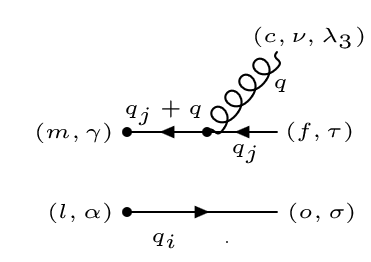
\includegraphics[width=0.85\textwidth]{images/qbargqM.png}
\end{figure}


\begin{figure}[h!]
\centering
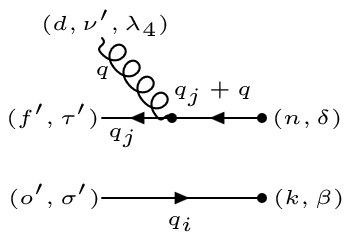
\includegraphics[width=0.85\textwidth]{images/qbargqMDega.png}
\end{figure}


\begin{figure}[h!]
\centering
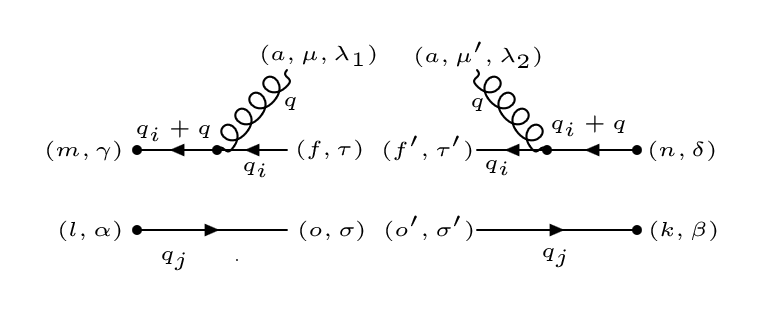
\includegraphics[width=0.85\textwidth]{images/qbargqMSquer.png}
\end{figure}
\newpage

\subsection{$M_1 {M_2}^{\dagger}$}

\begin{figure}[h!]
\centering
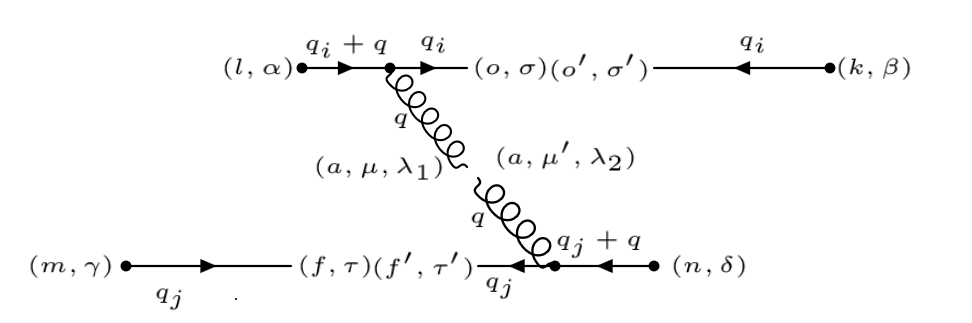
\includegraphics[width=0.85\textwidth]{images/M1M2Degaqqg.png}
\end{figure}

\subsection{$|M^{2}|$}

\begin{figure}[h!]
\centering
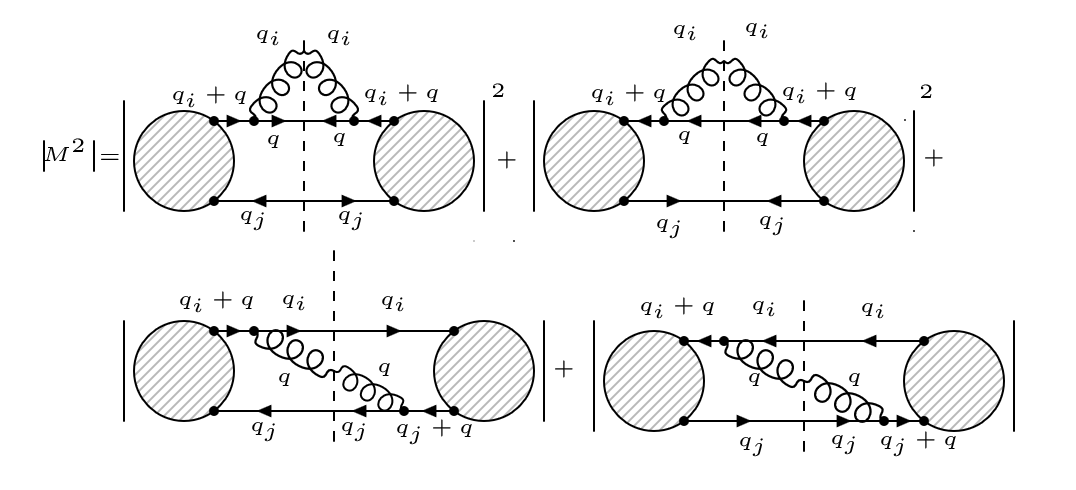
\includegraphics[width=0.85\textwidth]{images/qqgMSquer.png}
\end{figure}

\begin{figure}[h!]
\centering
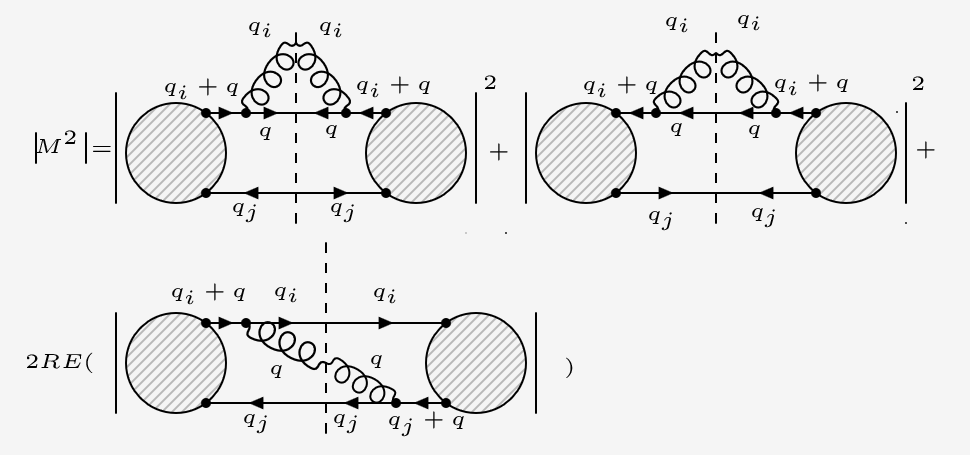
\includegraphics[width=0.85\textwidth]{images/REqqgMSquer.png}
\end{figure}

\newpage